\documentclass{article}
\usepackage{graphicx} % new way of doing eps files
\usepackage{listings} % nice code layout
\usepackage[usenames]{color} % color
\usepackage{float}
\definecolor{listinggray}{gray}{0.9}
\definecolor{graphgray}{gray}{0.7}
\definecolor{ans}{rgb}{1,0,0}
\definecolor{blue}{rgb}{0,0,1}
% \Verilog{title}{label}{file}
\newcommand{\Verilog}[3]{
  \lstset{language=Verilog}
  \lstset{backgroundcolor=\color{listinggray},rulecolor=\color{blue}}
  \lstset{linewidth=\textwidth}
  \lstset{commentstyle=\textit, stringstyle=\upshape,showspaces=false}
  \lstset{frame=tb}
  \lstinputlisting[caption={#1},label={#2}]{#3}
}


\author{Jiason Zhou and Jon Johnston}
\title{Lab 7: ALU and ALU Control}

\begin{document}
\maketitle

\section{Executive Summary}
The purpose of this lab is to design and simulate an ALU and an ALU Control. The ALU Control interprets the opcode and ALUOp signals, using them to generate a four-bit control singal that is sent to the ALU. The ALU itself does arithmetic and logic operations for the computer based on the control signal it receives. After running the test benches for the two modules, they generated the expected outputs, so the lab was successful.
\section{Test Report}
Verifying the operation of these modules required the use of two test benches, one for each of the modules.
\begin{enumerate}
	\item ALU Control Test
	\item ALU Test
\end{enumerate}

% This section should display the Expected Results Table and the Simulation Results for each test bench.  Make sure to label each figure correctly.  Please put them in the order of ERT1, SimResults1, ERT2, SimResults2 so that I can easily compare the ERT and Simulation Results.  To force the figures to be positioned correctly, add the float package (at the top of this file) and use the [H] after {figure} as I did below.  Also, if the ERT is on one page and the Simulation Results are on the next page, you can use a pagebreak as I did below so that the ERT goes to the next page also.

\pagebreak

\begin{figure}[H]
	\begin{center}
		\caption{Expected Results of the register test.}\label{fig:ert_registertest}
		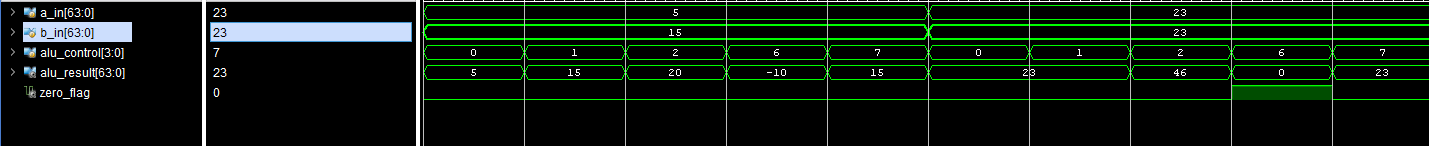
\includegraphics[width=1.0\textwidth]{../images/alu_test_timing_diagram.png}
	\end{center}
\end{figure}

\begin{figure}[H]
	\begin{center}
		\caption{Timing diagram for the register test.}\label{fig:registertest}
		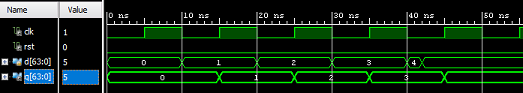
\includegraphics[width=1.0\textwidth]{../images/register_test_timing_diagram.png}
	\end{center}
\end{figure}


\section{Code Appendix}
% The code appendix should include the test bench code and module code for this lab.
\Verilog{Verilog code for testing a register.}{code:regtest}{../code/3_execute/alu.v}
\Verilog{Verilog code for implementing a register.}{code:reg}{../code/1_fetch/register.v}
\end{document} 